\documentclass[10pt,a4paper]{article}
\usepackage{amsmath}
\usepackage{amssymb}
\usepackage{graphicx}
\usepackage{color}
\usepackage{fancyhdr}
\usepackage{fancyvrb}
\usepackage[margin=3.5cm]{geometry}
\usepackage{framed}
\usepackage{enumerate}
\usepackage{textcomp}
\usepackage{float}
\def\ket#1{\left|#1\right\rangle}
\def\bra#1{\left\langle#1\right|}
\def\braket#1{\left\langle#1\right\rangle}

\definecolor{linkcol}{rgb}{0.0, 0.0, 0.7}
\usepackage[colorlinks=true,urlcolor=linkcol,citecolor=black,linkcolor=linkcol]{hyperref}

\renewcommand{\theequation}{11.\arabic{equation}}
\setcounter{section}{11}
\renewcommand\thesection{\arabic{section}}
\renewcommand\thesubsection{\thesection.\arabic{subsection}}

\fancyhf{}
\lhead{\tiny Y.~D.~Chong (2021)}
\rhead{\scriptsize MH2801: Complex Methods for the Sciences}
\lfoot{}
\rfoot{\thepage}
\pagestyle{fancy}

\begin{document}

\setcounter{page}{91}

\noindent
{\Large \textbf{11. Green's Functions}}
\vskip 0.2in

\label{greens-functions}

A \textbf{Green's function} is a solution to an inhomogenous
differential equation with a delta function ``driving term''.  It
provides a convenient method for solving more complicated inhomogenous
differential equations.  In physics, Green's functions methods are
used to describe a wide range of physical phenomena, such as the
response of mechanical systems to impacts or the emission of sound
waves from acoustic sources.

\subsection{The driven harmonic oscillator}
\label{the-driven-harmonic-oscillator}

As an introduction to the Green's function technique, we will study
the \textbf{driven harmonic oscillator}, which is a damped harmonic
oscillator subjected to an additional arbitrary driving force.  The
equation of motion is
\begin{align}
  \left[\frac{d^2}{dt^2} + 2 \gamma \frac{d}{dt} + \omega_0^2\right] x(t) = \frac{f(t)}{m}.
\end{align}
Here, $m$ is the mass of the particle, $\gamma$ is the damping
coefficient, and $\omega_0$ is the natural frequency of the
oscillator. The left side of the qquation is the same as in the damped
harmonic oscillator equation (see Chapter 5). On the right side, we
introduce a time-dependent driving force $f(t)$, which acts alongside
the pre-existing spring and damping forces. Given an arbitrarily
complicated $f(t)$, our goal is to determine $x(t)$.

\begin{figure}[ht]
  \centering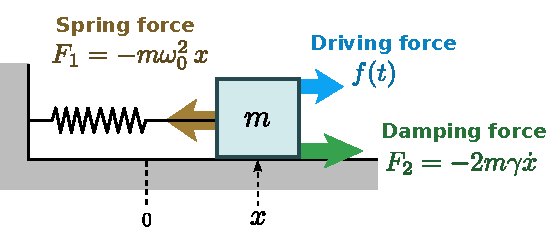
\includegraphics[width=0.6\textwidth]{oscillator_driven}
\end{figure}

\subsubsection{Green's function for the driven harmonic oscillator}
\label{greens-function-for-the-driven-harmonic-oscillator}

Prior to solving the driven harmonic oscillator problem for a general
driving force $f(t)$, let us first consider the following equation:
\begin{align}
  \left[\frac{\partial^2}{\partial t^2} + 2 \gamma \frac{\partial}{\partial t} + \omega_0^2\right] G(t, t') = \delta(t-t').
  \label{eq:greenfuneq}
\end{align}
The function $G(t,t')$, which depends on the two variables $t$ and
$t'$, is called the \textbf{Green's function}.  Note that the
differential operator on the left side involves only derivatives in
$t$.

The Green's function describes the motion of a damped harmonic
oscillator subjected to a particular driving force that is a delta
function (see Section 9.7), describing an infinitesimally sharp pulse
centered at $t = t'$:
\begin{align}
  \frac{f(t)}{m} = \delta(t-t').
\end{align}
Here's the neat thing about $G(t,t')$: once we know it, we can find a
specific solution to the driven harmonic oscillator equation for
\textit{any} $f(t)$.  The solution has the form
\begin{align}
  x(t) = \int^\infty_{-\infty} dt' \; G(t,t') \; \frac{f(t')}{m}.
\end{align}
To show that this is indeed a solution, plug it into the equation of
motion:
\begin{align}
  \left[\frac{d^2}{dt^2} + 2 \gamma \frac{d}{dt} + \omega_0^2\right]\, x(t) &= \int^\infty_{-\infty} dt' \; \left[\frac{\partial^2}{\partial t^2} + 2 \gamma \frac{\partial}{\partial t} + \omega_0^2\right] G(t,t') \frac{f(t')}{m} \\
  &= \int^\infty_{-\infty} dt' \; \delta(t-t')\, \frac{f(t')}{m} \\
  &= \frac{f(t)}{m}.
\end{align}
Note that we can move the differential operator inside the integral
because $t$ and $t'$ are independent variables.

The Green's function concept is based on the principle of
superposition.  The motion of the oscillator is induced by the driving
force, but the value of $x(t)$ at time $t$ does not depend only on the
instantaneous value of $f(t)$ at time $t$; instead, it depends on the
values of $f(t')$ over all past times $t' < t$. We can thus decompose
$f$ into a superposition of pulses described by delta functions at
different times. Then $x(t)$ is a superposition of the oscillations
produced by the individual pulses.

\subsubsection{Finding the Green's function}
\label{finding-the-greens-function}

To find the Green's function, we can use the Fourier transform
(Chapter 10).  Let us assume that the Fourier transform of $G(t,t')$
with respect to $t$ is convergent, and that the oscillator is not
critically damped (i.e., $\omega_0 \ne \gamma$; see Section
4.3.3). The Fourier transformation of the Green's function (also
called the \textbf{frequency-domain Green's function}) is
\begin{align}
  G(\omega, t') = \int_{-\infty}^\infty dt \; e^{i\omega t}\, G(t,t').
\end{align}
Here, we have used the sign convention for time-domain Fourier
transforms (see Section 9.3).  Applying the Fourier transform to both
sides of the Green's function equation, we get
\begin{align}
  \left[- \omega^2 - 2i \gamma\omega + \omega_0^2\right] G(\omega,t') = \int_{-\infty}^\infty dt \; e^{i\omega t}\, \delta(t-t') = e^{i\omega t'}.
\end{align}
The differential equation for $G(t,t')$ has thus been converted into
an \textit{algebraic} equation for $G(\omega,t')$, whose solution is
\begin{align}
  G(\omega, t') = - \frac{e^{i\omega t'}}{\omega^2 + 2i\gamma\omega - \omega_0^2}.
\end{align}
Finally, we retrieve the time-domain solution by using the inverse
Fourier transform:
\begin{align}
  G(t,t') &= \int_{-\infty}^\infty \frac{d\omega}{2\pi} \, e^{-i\omega t} G(\omega, t')  \\
  &= - \int_{-\infty}^\infty \frac{d\omega}{2\pi} \, \frac{e^{-i\omega (t-t')}}{\omega^2 + 2i\gamma\omega - \omega_0^2}.
\end{align}
The denominator of the integral is a quadratic expression, so this can
be re-written as:
\begin{align}
  G(t,t') = - \int_{-\infty}^\infty \frac{d\omega}{2\pi} \, \frac{e^{-i\omega (t-t')}}{(\omega - \omega_+)(\omega - \omega_-)} \quad\mathrm{where}\;\; \omega_{\pm} = -i\gamma \pm \sqrt{\omega_0^2-\gamma^2}.
\end{align}
This can be evaluated by contour integration.  The integrand has two
poles, which are precisely the complex frequencies of the damped
harmonic oscillator; both lie in the negative complex plane.  For $t <
t'$, Jordan's lemma requires us to close the contour in the upper
half-plane, enclosing neither pole, so the integral is zero.  For $t >
t'$, we must close the contour in the lower half-plane, enclosing both
poles, so the result is
\begin{align}
  G(t,t') &= i \Theta(t-t') \, \left[ \frac{e^{-i\omega_+ (t-t')}}{\omega_+ - \omega_-
    } + \frac{e^{-i\omega_- (t-t')}}{\omega_- - \omega_+}\right] \\
  &= \Theta(t-t') \;e^{-\gamma(t-t')} \; \times \left\{\begin{array}{ll} \frac{1}{\sqrt{\omega_0^2-\gamma^2}}\, \sin\left[\sqrt{\omega_0^2-\gamma^2} (t-t')\right], & \gamma < \omega_0, \\
  \frac{1}{\sqrt{\gamma^2-\omega_0^2}}\, \sinh\left[\sqrt{\gamma^2-\omega_0^2} (t-t')\right], & \gamma > \omega_0.\end{array}\right.
\end{align}
Here, $\Theta(t-t')$ refers to the step function
\begin{align}
  \Theta(\tau) = \left\{\begin{array}{ll} 1, &\;\;\;\textrm{for} \; \tau \ge 0\\ 0,&\;\;\; \textrm{otherwise.}\end{array}\right.
\end{align}
This result is plotted below. The solution for the critically damped
case, $\gamma = \omega_0$, is left as an exercise.

\begin{figure}[ht]
  \centering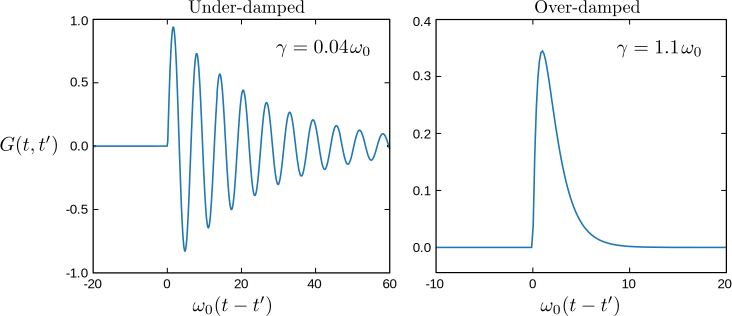
\includegraphics[width=0.9\textwidth]{oscillator_greenfun}
\end{figure}

\subsubsection{Features of the Green's function}
\label{features-of-the-greens-function}

The time-domain Green's function represents the motion of the
oscillator in response to a pulse of force, $f(t) = m\,
\delta(t-t')$. Let us examine its features in greater detail.

The first thing to notice is that the Green's function depends on $t$
and $t'$ only in the combination $t-t'$. This makes sense: the
response of the oscillator to the force pulse should only depend on
the time elapsed since the pulse. We can exploit this property by
re-defining the frequency-domain Green's function as
\begin{align}
  G(\omega) = \int_{-\infty}^\infty dt \; e^{i\omega (t-t')}\, G(t-t'),
\end{align}
which then obeys
\begin{align}
  \left[- \omega^2 - 2i \gamma\omega + \omega_0^2\right] G(\omega) = 1.
\end{align}
This is nicer to work with, as there is no extraneous $t'$ variable
present.

Next, note how the Green's function behaves just before and after the
pulse. Its value is zero for all $t - t' < 0$ (i.e., prior to the
pulse). This feature will be discussed in greater detail in the next
section. Moreover, there is no discontinuity in $x(t)$ at $t - t' =
0$; the force pulse does not cause the oscillator to ``teleport''
instantaneously to a different position.  Instead, it produces a
discontinuity in the oscillator's velocity.

We can calculate the velocity discontinuity by integrating the Green's
function equation over an infinitesimal interval of time surrounding
$t'$:
\begin{align}
  \lim_{\epsilon \rightarrow 0} \int_{t'-\epsilon}^{t'+\epsilon} dt \left[\frac{\partial^2}{\partial t^2} + 2\gamma\frac{\partial}{\partial t} + \omega_0^2\right] G(t,t') &= \lim_{\epsilon \rightarrow 0} \int_{t'-\epsilon}^{t'+\epsilon} dt \; \delta(t-t') \\
  = \lim_{\epsilon \rightarrow 0} \left\{ \left.\frac{\partial G(t,t')}{\partial t}\right|_{t = t' +\epsilon} - \left.\frac{\partial G(t,t')}{\partial t}\right|_{t = t' - \epsilon}\right\} &= 1.
\end{align}
On the last line, the expression on the left-hand side represents the
difference between the velocities just after and before the
pulse. Evidently, the pulse imparts one unit of velocity at $t=t'$.
Looking at the solutions obtained in
Section~\ref{finding-the-greens-function}, we can verify that indeed
$\partial G/\partial t = 0$ right before the pulse, and $\partial
G/\partial t = 1$ right after it.

For $t - t' > 0$, the applied force goes back to zero, and the system
behaves like the undriven harmonic oscillator.  If the oscillator is
under-damped ($\gamma < \omega_0$), it undergoes a decaying
oscillation around the origin.  If the oscillator is over-damped
($\gamma > \omega_0$), it moves ahead for some distance, then settles
exponentially back to the origin.

\subsubsection{Causality}
\label{causality}

We have seen that the motion $x(t)$ ought to depend on the driving
force $f(t')$ at all past times $t' < t$, but should \textit{not}
depend on the force at future times.  Because of the relation
\begin{align}
  x(t) = \int_{-\infty}^\infty dt'\; G(t,t')\, \frac{f(t')}{m},
\end{align}
this means that the Green's function ought to satisfy
\begin{align}
  G(t,t') = 0 \;\; \mathrm{for}\;\; t -t' < 0.
\end{align}
This condition is referred to as \textbf{causality}, because it is
equivalent to saying that \textit{cause} must precede \textit{effect}.
A Green's function with this feature is called a \textbf{causal
  Green's function}.

For the driven harmonic oscillator, the time-domain Green's function
satisfies a second-order differential equation, so its general
solution must contain two free parameters.  The specific solution we
derived in Section~\ref{finding-the-greens-function} turns out to be
the \textit{only} causal solution. There are a couple of ways to see
why.

The first way is to observe that for $t > t'$, the Green's function
satisfies the differential equation for the \textit{undriven} harmonic
oscillator. But based on the discussion in
Section~\ref{features-of-the-greens-function}, the causal Green's
function needs to obey two conditions at $t = t' + 0^+$: (i) $G = 0$,
and (ii) $\partial G / \partial t = 1$. These act as two boundary
conditions for the undriven harmonic oscillator equation, giving rise
to the specific solution that we found.

The other way to see that the causal Green's function is unique is to
imagine adding to our specific solution any solution $x_1(t)$ for the
undriven harmonic oscillator.  It is easily verified that the
resulting $G(t,t')$ is also a solution to the Green's function
equation \eqref{eq:greenfuneq}. Since the general solution for
$x_1(t)$ contains two free parameters, we have thus found the general
solution for $G(t,t')$. But the solutions for $x_1(t)$ are all
infinite in the $t \rightarrow -\infty$ limit, \textit{except} for the
trivial solution $x_1(t) = 0$. That choice corresponds to the causal
Green's function we found.

\subsection{Space-time Green's functions (optional topic)}
\label{space-time-greens-functions}

The Green's function method can also be used for studying waves. For
simplicity, we restrict the following discussion to waves propagating
through a uniform medium. Also, we will just consider 1D space; the
generalization to higher spatial dimensions is straightforward.

As discussed in Chapter 6, wave propagation can be modelled by the
wave equation
\begin{align}
  \left[\frac{\partial^2}{\partial x^2} - \frac{1}{c^2} \frac{\partial^2}{\partial t^2} \right] \psi(x,t) = 0,
\end{align}
where $\psi(x,t)$ is a complex wavefunction and $c$ is the wave
speed. Henceforth, to simplify the equations, we will set $c = 1$.
(You can reverse this simplification by replacing all instances of $t$
with $c t$, and $\omega$ with $\omega/c$, in the subsequent formulas.)

The wave equation describes how waves propagate \textit{after} they
have already been created. To describe how the waves are generated in
the first place, we must modify the wave equation by introducing a
term on the right-hand side, called a \textbf{source}:
\begin{align}
  \left[\frac{\partial^2}{\partial x^2} - \frac{\partial^2}{\partial t^2} \right] \psi(x,t)\, = f(x,t).
\end{align}
The source term turns the wave equation into an inhomogenous partial
differential equation, similar to the driving force for the driven
harmonic oscillator.

\subsubsection{Time-domain Green's function (optional topic)}
\label{time-domain-greens-function}

The wave equation's \textbf{time-domain Green's function} is defined
by setting the source term to delta functions in both space and time:
\begin{align}
  \left[\frac{\partial^2}{\partial x^2} - \frac{\partial^2}{\partial t^2} \right] G(x,x';t-t') = \delta(x-x')\, \delta(t-t').
\end{align}
Here $G$ is a function of two spatial variables, $x$ and $x'$, as well
as two temporal variables $t$ and $t'$.  It corresponds to the wave
generated by a pulse
\begin{align}
  f(x,t) = \delta(x-x')\,\delta(t-t').
\end{align}
The differential operator in the Green's function equation only
involves $x$ and $t$, so we can regard $x'$ and $t'$ as parameters
specifying where the pulse is localized in space and time.  This
Green's function ought to depend on the time variables only in the
combination $t-t'$, as we saw in
Section~\ref{features-of-the-greens-function}. To emphasize this, we
have written it as $G(x,x';t-t')$.

The Green's function describes how a source localized at a space-time
point influences the wavefunction at other positions and times. Once
we have found the Green's function, it can be used to construct
solutions for arbitrary sources:
\begin{align}
  \psi(x,t) = \int dx' \,\int_{-\infty}^\infty dt'\; G(x,x';t-t') \, f(x', t').
\end{align}

\subsubsection{Frequency-domain Green's function (optional topic)}
\label{frequency-domain-greens-function}

The \textbf{frequency-domain Green's function} is obtained by Fourier
transforming the time-domain Green's function in the $t-t'$
coordinate:
\begin{align}
  G(x,x';\omega) = \int_{-\infty}^\infty d\tau\; e^{i\omega \tau}\, G(x,x'; \tau).
\end{align}
It obeys the differential equation
\begin{align}
  \left[\frac{\partial^2}{\partial x^2} + \omega^2 \right] G(x,x';\omega) = \delta(x-x').
\end{align}
Just as we can write the time-domain solution to the wave equation in
terms of the time-domain Green's function, we can do the same for the
frequency-domain solution:
\begin{align}
  \Psi(x,\omega) = \int dx' \; G(x,x';\omega) \, F(x', \omega),
\end{align}
where
\begin{align}
  \Psi(x,\omega) = \int_{-\infty}^\infty dt \; e^{i\omega t} \, \psi(x,t), \quad F(x,\omega) = \int_{-\infty}^\infty dt \; e^{i\omega t} \, f(x,t).
\end{align}

\subsubsection{Outgoing boundary conditions (optional topic)}
\label{outgoing-boundary-conditions}

So far, we have not specified the boundary conditions along $x$. There
are several possible choices of boundary conditions, corresponding to
different physical scenarios.  For example, if the waves are trapped
within a finite domain $x \in (x_a,x_b)$, with reflecting walls, we
would impose Dirichlet boundary conditions: $G(x,x';\omega) = 0$ for
$x,x' \in \{ x_a, x_b\}$.

We will focus on the interesting case of an unbounded spatial domain:
$x \in (-\infty, \infty)$. This describes, for example, the case of a
loudspeaker emitting sound waves into an infinite empty space. The
relevant boundary conditions for this case are called \textbf{outgoing
  boundary conditions}.  The Green's function should correspond to a
left-moving wave for $x$ to the left of the source, and to a
right-moving wave for $x$ to the right of the source.

We can guess the form of the Green's function obeying these boundary
conditions:
\begin{align}
  G(x,x';\omega) = \left\{\begin{array}{ll}A \, e^{-i\omega (x-x')}, & x \le x', \\ B \, e^{i\omega (x-x')}, & x \ge x'\end{array}\right. \quad \mathrm{for}\;\mathrm{some}\;\; A, B \in \mathbb{C}.
\end{align}
It is straightforward to verify that this formula for $G(x,x',\omega)$
satisfies the wave equation in both the regions $x < x'$ and $x > x'$,
as well as satisfying outgoing boundary conditions.  To determine the
$A$ and $B$ coefficients, note that $G(x,x')$ should be continuous at
$x = x'$, so $A = B$. Then, integrating the Green's function equation
across $x'$ gives
\begin{align}
  \lim_{\epsilon \rightarrow 0} \int_{x'-\epsilon}^{x'+\epsilon} \left[\frac{\partial^2}{\partial x^2} + \omega^2\right]G(x-x') &= \lim_{\epsilon \rightarrow 0} \int_{x'-\epsilon}^{x'+\epsilon} \delta(x-x') \\
  = \lim_{\epsilon \rightarrow 0} \left\{ \left.\frac{\partial G}{dx} (x,x') \right|_{x = x'+\epsilon} - \left.\frac{\partial G}{\partial x} (x,x') \right|_{x = x'-\epsilon}\right\} &= i\omega (B + A) = 1.
\end{align}
Combining these two equations gives $A = B = 1/2i\omega$.  Hence,
\begin{align}
  G(x,x';\omega) = \frac{e^{i\omega |x-x'|}}{2i\omega}.
\end{align}

\subsection{Causality and the time-domain Green's function (optional topic)}
\label{causality-and-the-time-domain-greens-function}

Let us try converting the above result into a time-domain Green's
function by using the inverse Fourier transform:
\begin{align}
  G(x,x';t-t') &= \int_{-\infty}^\infty \frac{d\omega}{2\pi} \, e^{-i\omega (t-t')} \, G(x,x'; \omega) \\
  &= \int_{-\infty}^\infty d\omega \, \frac{e^{i\omega \left[|x-x'| - (t-t')\right]}}{4\pi i\omega}\qquad (?!?)
\end{align}
There is a problem: the integral runs over the real-$\omega$ line, yet
the integrand has a pole at $\omega = 0$, on the real axis, making the
integral ill-defined.

To resolve this, we redefine $G(x,x';\omega)$ as an integral over a
\textit{deformed} contour $\Gamma$:
\begin{align}
  G(x,x';t-t') \equiv \int_\Gamma d\omega \, \frac{e^{i\omega \left[|x-x'| - (t-t')\right]}}{4\pi i\omega}.
\end{align}
We will choose to deform the contour in a very specific way, which
turns out to be the choice that satisfies causality
(Section~\ref{causality}).  As shown in the left subplot of the figure
below, it runs along the real axis, but skips \textit{above} the pole
at the origin.

\begin{figure}[ht]
  \centering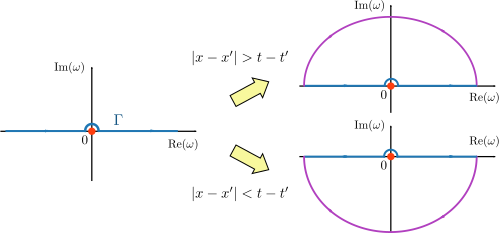
\includegraphics[width=0.9\textwidth]{causality_contour}
\end{figure}

The integral can be solved by either closing the contour in the upper
half-plane, or in the lower half-plane. If we close the contour above,
then the loop contour does not enclose the pole, and hence
$G(x,x';t-t') = 0$. According to Jordan's lemma, we must do this if
the exponent in the integrand obeys
\begin{align}
  |x-x'| - (t-t') > 0  \quad \Rightarrow \quad |x-x'| > t-t'.
\end{align}
This inequality is satisfied in two cases: either (i) $t < t'$ (in
which case the inequality is satisfied for all $x,x'$ because $|x-x'|$
is strictly non-negative), or (ii) $t > t'$ but the value of $t-t'$ is
smaller than $|x-x'|$.  To understand the physical meaning of these
two cases, recall that $G(x,x';t-t')$ represents the field at position
$x$ and time $t$ resulting from a pulse at the space-time point
$(x',t')$.  Thus, case (i) corresponds to times occurring before the
pulse, and case (ii) corresponds to times occurring after the pulse
but too far away from the pulse location for a wave to reach in time.

For the other case, $|x-x'| - (t-t') < 0$, the residue theorem gives
\begin{align}
  G(x,x';t-t') = -1/2.
\end{align}
The space-time diagram below summarizes the results:

\begin{figure}[ht]
  \centering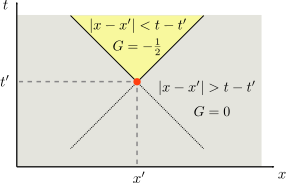
\includegraphics[width=0.55\textwidth]{spacetime_diagram}
\end{figure}

The resulting time-domain wavefunctions can be written as
\begin{align}
  \psi(x,t) = \int_{-\infty}^\infty dx' \int_{-\infty}^\infty dt' \left[-\frac{1}{2}\,\Theta(t-t' - |x-x'|)\right] f(x',t'),
\end{align}
where $\Theta$ denotes the unit step function.  In other words, the
wavefunction at each space-time point $(x,t)$ receives equal
contribution from the sources $f(x',t')$ at space-time points
$(x',t')$ lying within the ``past light cone''.

\subsection{Looking ahead (optional topic)}\label{looking-ahead}

Green's functions are widely used in the study of acoustic and
electromagnetic waves, which is a vast topic covered in advanced
courses in theoretical physics, electrical engineering, and mechanical
engineering. Here, we give a brief sketch of some future directions of
study.

So far, we have focused our attentions on the simplest case of an
infinite one-dimensional uniform medium. Most practical applications
are concerned with three spatial dimensions and non-uniform media. For
such cases, the wave equation's frequency-domain Green's function can
be generalized to
\begin{align}
  \left[\nabla^2 + n^2(\vec{r}) \, \left(\frac{\omega}{c}\right)^2\right]\, G(\vec{r},\vec{r}';\omega) = \delta^3(\vec{r}-\vec{r}'),
\end{align}
where $\nabla^2 = \partial^2/\partial x^2 + \partial^2/\partial y^2 +
\partial^2/\partial z^2$ is the three-dimensional Laplacian operator,
and $n(\vec{r})$ is a space-dependent refractive index (see Section
5.5.1). On the right-hand side of this equation is the
three-dimensional delta function (see Section 9.8), which describes a
point source located at position $\vec{r}'$ in the three-dimensional
space.

When $n = 1$, the above equation is similar to the frequency-domain
Green's function equation studied in
Section~\ref{outgoing-boundary-conditions}, except that the problem is
three-dimensional rather than one-dimensional. Again assuming outgoing
boundary conditions, the Green's function in three dimensions can be
found using contour integrals similar to those we have previously
covered; the result is
\begin{align}
  G(\vec{r},\vec{r}';\omega) = -\frac{e^{i(\omega/c)|\vec{r}-\vec{r}'|}}{4\pi|\vec{r}-\vec{r}'|}.
\end{align}
Like the Green's function in one dimension, this depends on
$|\vec{r}-\vec{r}'|$, and thence describes waves that are emitted
isotropically from the source at $\vec{r}'$. However, the magnitude of
$G$ now decreases to zero with distance, due to the
$|\vec{r}-\vec{r}'|$ in the denominator. This matches our everyday
experience that the sound emitted from a point source grows fainter
with distance, which is because the energy carried by the outgoing
wave is spread out over a larger area with increasing distance from
the source. This is unlike waves in one-dimensional space, which do
not become weaker with distance.

When $n(\vec{r})$ is not a constant but varies with position
$\vec{r}$, then the waves emitted by the source do not radiate
outwards in a simple way. The variations in the refractive index cause
the waves to scatter in complicated ways. In most situations, the
exact solution for the Green's function cannot be obtained
analytically, but must be computed using specialized numerical
methods.

For electromagnetic waves, there is another important complication
coming from the fact that electromagnetic fields are described by
vectors (i.e., the electric field vector and the magnetic field
vector), not scalars.  The propagation of electromagnetic waves is
therefore described by a vectorial wave equation, not the scalar wave
equation that we have looked at so far. Moreover, electromagnetic
waves are not generated by scalar sources, but by vector sources
(typically, electrical currents). The corresponding Green's function
is not a scalar function, but a multi-component entity called a
\textbf{dyadic Green's function}, which describes the vector waves
emitted by a vector source.

Finally, even though we have dealt so far with classical (non-quantum)
waves, the Green's function concept extends to the theory of quantum
mechanics. In quantum field theory, which is the principal theoretical
framework used in fundamental physics, calculations typically involve
quantum mechanical generalizations of the Green's functions we have
studied above, whose values are no longer simple numbers but rather
quantum mechanical operators.

\clearpage
\subsection{Exercises}\label{exercises}

\begin{enumerate}
\item
  Find the time-domain Green's function of the critically-damped
  harmonic oscillator ($\gamma = \omega_0$).
\item
  Consider an overdamped harmonic oscillator ($\gamma > \omega_0$)
  subjected to a \emph{random} driving force $f(t)$, which fluctuates
  between random values, which can be either positive or negative, at
  each time $t$. The random force satisfies
  \begin{equation}
    \left\langle f(t)\right\rangle = 0 \quad\mathrm{and}\;\;\;\left\langle f(t) f(t')\right\rangle = A \, \delta(t-t'),
  \end{equation}
  where $\left\langle\cdots\right\rangle$ denotes an average taken
  over many realizations of the random force and $A$ is some constant.
  Using the causal Green's function, find the correlation function
  $\left\langle x(t_1)\, x(t_2) \right\rangle$ and the mean squared
  deviation $\left\langle [x(t+\Delta t) - x(t)]^2 \right\rangle.$
  \vskip -0.05in
  \hfill{\scriptsize [solution~available]}
\end{enumerate}

\end{document}
